% Original vector diagram corresponding to source Fig.25.3, PDF113 / printed101.
% Physical chi momenta: p1,p2 enter, p3,p4 leave; q=p1+p2=p3+p4 and s=-q^2.
% Both circles are full phi-chi-chi kernels. The DOUBLE DASHED stroke is ONE
% resummed phi propagator, not two internal edges. No chi exchange is present.
% These added labels explain the source's originally unlabeled exchange graph.
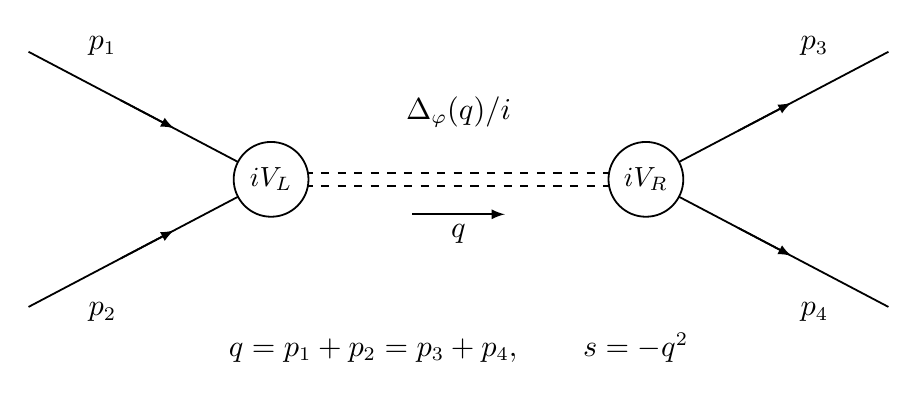
\begin{tikzpicture}[x=14mm,y=12mm,line width=.65pt,>=latex,
  font=\fontsize{10.5}{12}\selectfont,
  kernel/.style={circle,draw,fill=white,minimum size=9.5mm,
    inner sep=1pt,font=\fontsize{10}{11}\selectfont}]
  \def\cxxvflow#1#2#3#4{%
    \draw (#1,#2) -- (#3,#4);
    \draw[->] ({.62*(#1)+.38*(#3)},{.62*(#2)+.38*(#4)})
      -- ({.40*(#1)+.60*(#3)},{.40*(#2)+.60*(#4)});
  }
  \cxxvflow{-3.9}{1.35}{-1.7}{0}
  \cxxvflow{-3.9}{-1.35}{-1.7}{0}
  \cxxvflow{1.7}{0}{3.9}{1.35}
  \cxxvflow{1.7}{0}{3.9}{-1.35}
  \draw[dashed] (-1.7,.070) -- (1.7,.070);
  \draw[dashed] (-1.7,-.070) -- (1.7,-.070);
  \node[kernel] at (-1.7,0) {$iV_L$};
  \node[kernel] at (1.7,0) {$iV_R$};
  \node[above] at (0,.44) {$\symbf{\Delta}_\varphi(q)/i$};
  \draw[->] (-.42,-.37) -- (.42,-.37);
  \node[below] at (0,-.37) {$q$};
  \node[above] at (-3.23,1.20) {$p_1$};
  \node[below] at (-3.23,-1.20) {$p_2$};
  \node[above] at (3.23,1.20) {$p_3$};
  \node[below] at (3.23,-1.20) {$p_4$};
  \node at (0,-1.78) {$q=p_1+p_2=p_3+p_4,\qquad s=-q^2$};
\end{tikzpicture}
